\section{Markov chain VS Simulation}

\subsection{Example model}
Consider the Markov chain paradigm in figure \ref{Model_mini}. The illustrated model represents the unrealistically small system of a hospital with a system capacity of five and an ambulance parking capacity of three. The hospital in this particular example also has four servers and a threshold of three; meaning that every ambulance that arrives in a time that there are three or more individuals in the hospital, will proceed to the parking space.

\begin{figure}[h]
    \centering
    \begin{tikzpicture}[-, node distance = 1cm, auto]
        \node[state] (empty) {(0,0)};
        \node[state, right=of empty] (one) {(0,1)};
        \node[state, right=of one] (two) {(0,2)};
        \node[state, right=of two] (three) {(0,3)};
        \node[state, right=of three] (four) {(0,4)};
        \node[state, right=of four] (five) {(0,5)};

        \node[state, below=of three] (three_one) {(1,3)};
        \node[state, below=of three_one] (three_two) {(2,3)};
        \node[state, below=of four] (four_one) {(1,4)};
        \node[state, below=of four_one] (four_two) {(2,4)};
        \node[state, below=of five] (five_one) {(1,5)};
        \node[state, below=of five_one] (five_two) {(2,5)};

        \draw[every loop]
            (empty) edge[bend left] node {\( \Lambda \)} (one)
            (one) edge[bend left] node {\( \mu \)} (empty)
            (one) edge[bend left] node {\( \Lambda \)} (two)
            (two) edge[bend left] node {\( 2 \mu \)} (one)
            (two) edge[bend left] node {\( \Lambda \)} (three)
            (three) edge[bend left] node {\( 3 \mu \)} (two)
            (three) edge[bend left] node {\( \lambda^o \)} (four)
            (four) edge[bend left] node {\( 4 \mu \)} (three)
            (four) edge[bend left] node {\( \lambda^o \)} (five)
            (five) edge[bend left] node {\( 4 \mu \)} (four)
            (three) edge[bend left] node {\( \lambda^A \)} (three_one)
            (three_one) edge[bend left] node {\( 3 \mu \)} (three)
            (three_one) edge[bend left] node {\( \lambda^o \)} (four_one)
            (four_one) edge[bend left] node {\( 4 \mu \)} (three_one)
            (four_one) edge[bend left] node {\( \lambda^o \)} (five_one)
            (five_one) edge[bend left] node {\( 4 \mu \)} (four_one)
            (four) edge node {\( \lambda^A \)} (four_one)
            % (four_one) edge[bend left] node {\( \mu \)} (four)
            (five) edge node {\( \lambda^A \)} (five_one)
            % (five_one) edge[bend left] node {\( \mu \)} (five)
            (three_one) edge[bend left] node {\( \lambda^A \)} (three_two)
            (three_two) edge[bend left] node {\( 3 \mu \)} (three_one)
            (four_one) edge node {\( \lambda^A \)} (four_two)
            % (four_two) edge[bend left] node {\( \mu \)} (four_one)
            (five_one) edge node {\( \lambda^A \)} (five_two)
            % (five_two) edge[bend left] node {\( \mu \)} (five_one)
            (three_two) edge[bend left] node {\( \lambda^o \)} (four_two)
            (four_two) edge[bend left] node {\( 4 \mu \)} (three_two)
            (four_two) edge[bend left] node {\( \lambda^o \)} (five_two)
            (five_two) edge[bend left] node {\( 4 \mu \)} (four_two)
            ;       
    \end{tikzpicture}
    \caption{Markov chains: number of servers=4} 
    \label{Model_mini}
\end{figure}

In addition to the Markov chain model a simulation model has also been built based on the same parameters. Comparing the results of the Markov model and the equivalent simulation model the resultant plots arose.

\begin{figure}
    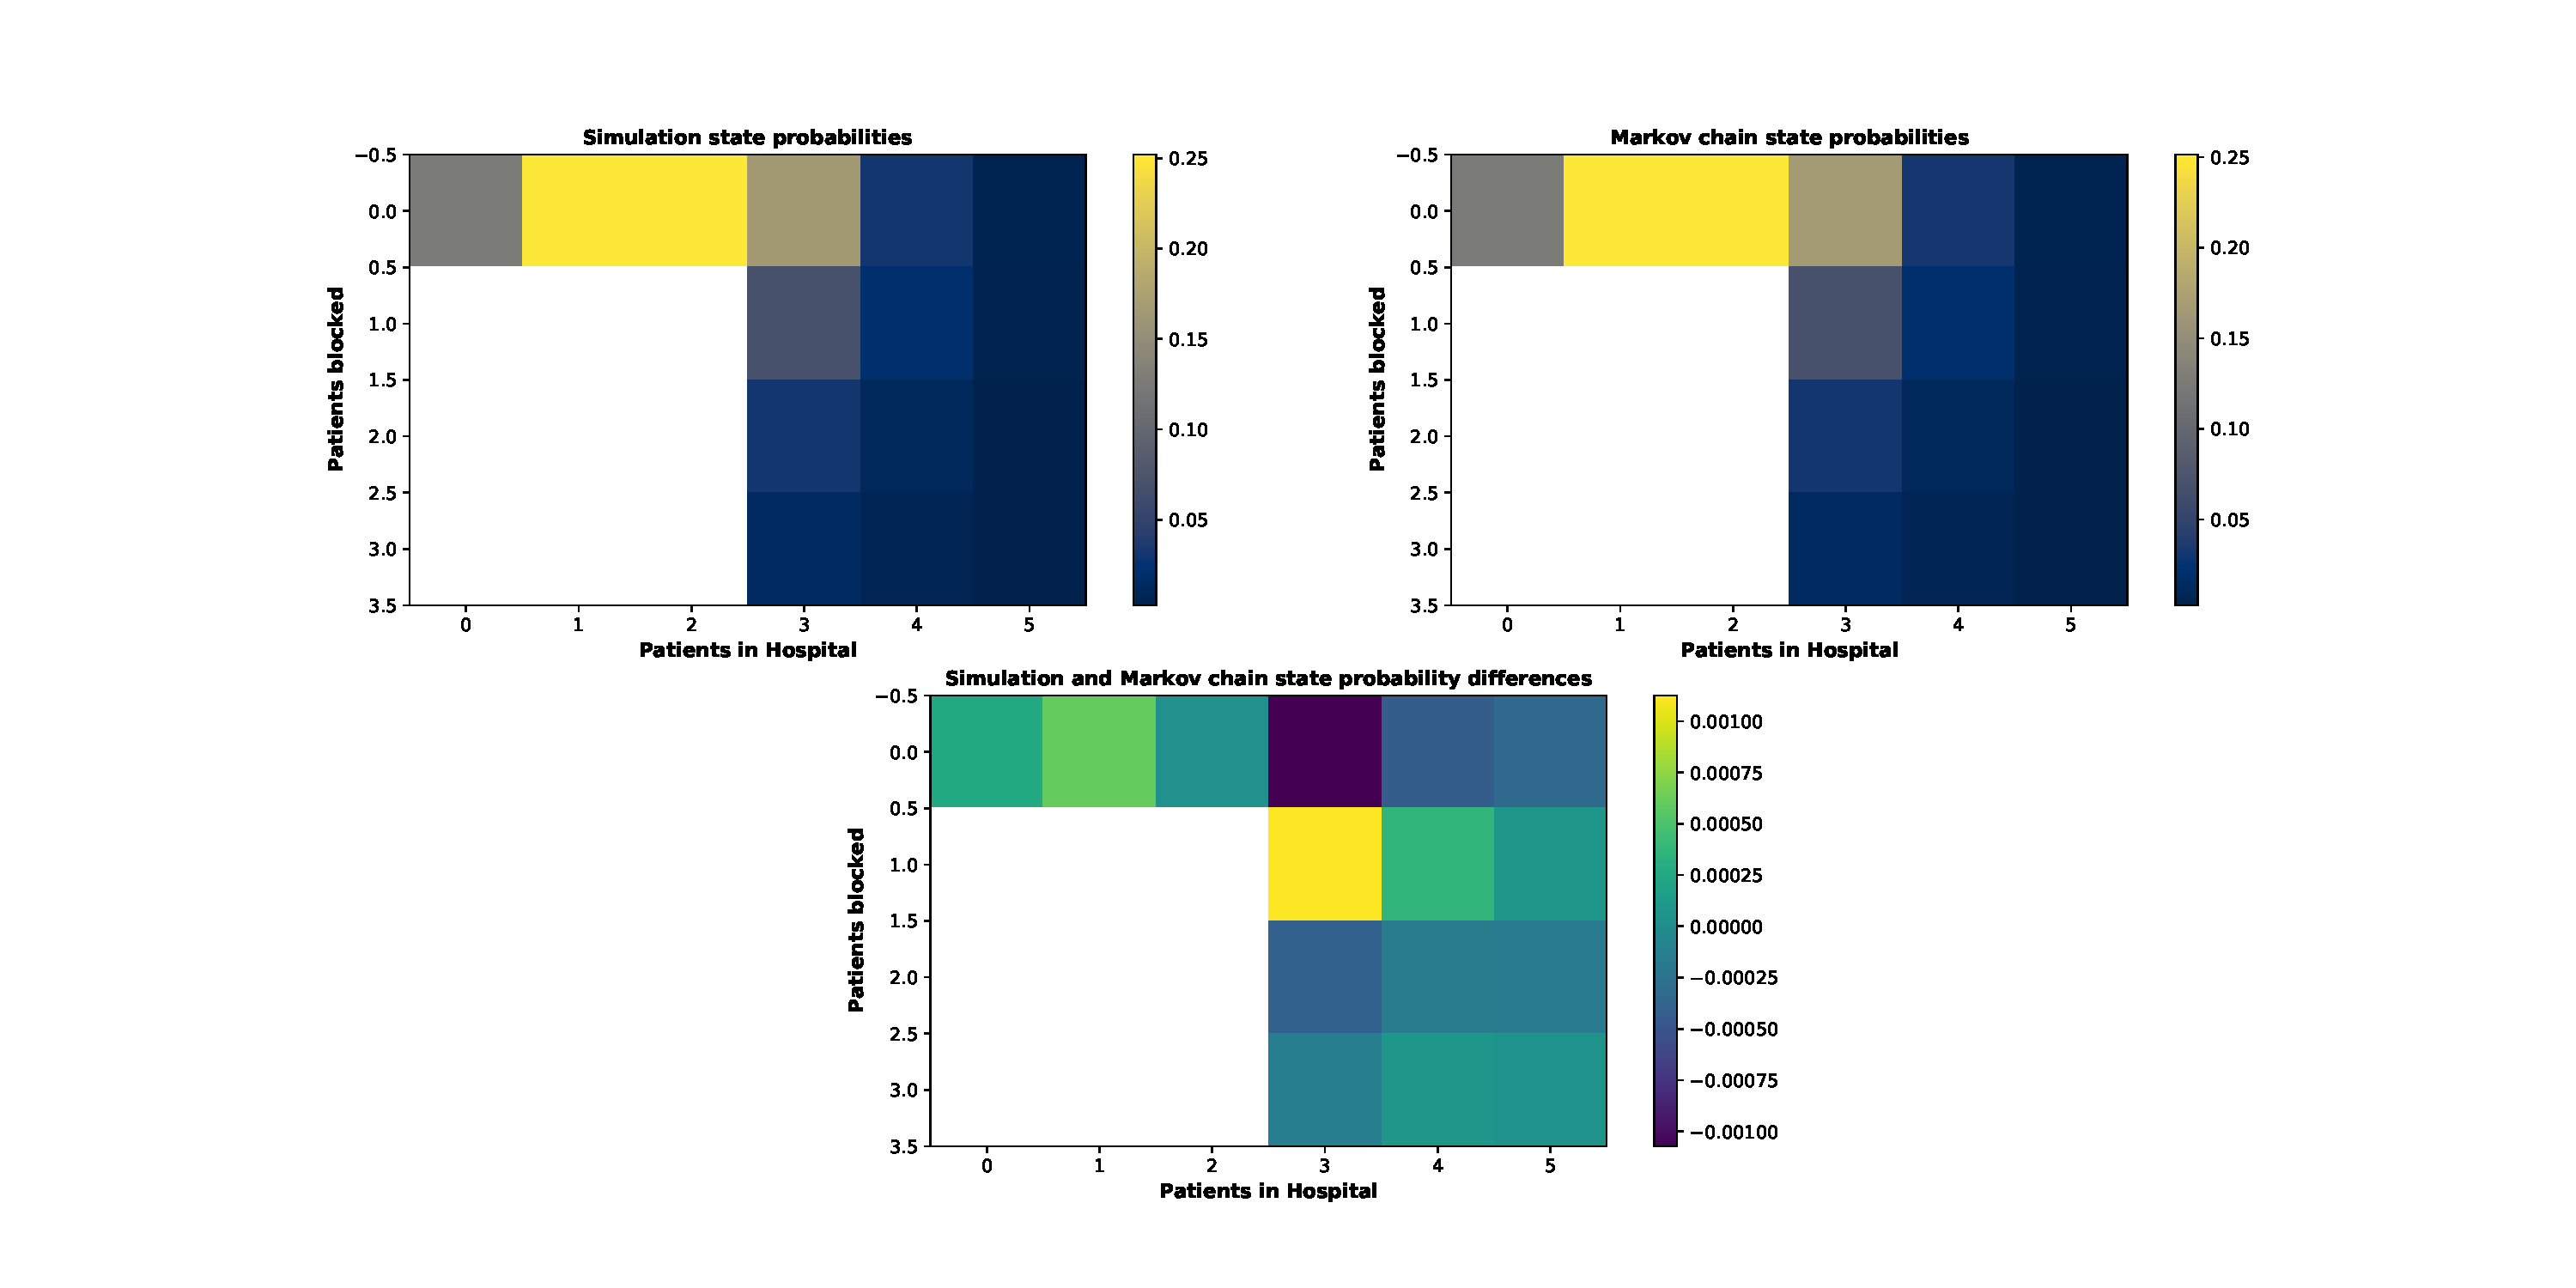
\includegraphics[width=\linewidth]{Comparisons/Example_model/Heatmap/main.pdf}
    \caption{Heatmaps of Simulation, Markov chains and differences of the two}
    \label{Heatmap_mini}
\end{figure}

The heatmaps in figure \ref{Heatmap_mini} represent the state probabilities for the Markov chain model, the simulation model and the difference between the two. Each pixel of the heatmap corresponds to the equivalent state of figure \ref{Model_mini} and represents the probability of being at that state in any particular moment of time.

It can be observed that both Markov chain and simulation models' state probabilities vary from 5\% to 25\% and that states \( (0, 1) \) and \( (0, 2) \) are the most visited ones. Looking at the differences' heatmap, one may identify that the differences between the two are minimal.

